\documentclass[conference]{IEEEtran}
\IEEEoverridecommandlockouts
% The preceding line is only needed to identify funding in the first footnote. If that is unneeded, please comment it out.
\usepackage{cite}
\usepackage{amsmath,amssymb,amsfonts}
\usepackage{algorithmic}
\usepackage{graphicx}
\usepackage{textcomp}
\usepackage{xcolor}
\def\BibTeX{{\rm B\kern-.05em{\sc i\kern-.025em b}\kern-.08em
    T\kern-.1667em\lower.7ex\hbox{E}\kern-.125emX}}
\begin{document}

\title{FedGuard: A Governance Framework for Secure and Regulation-Compliant Federated Learning\\}

\author{\IEEEauthorblockN{Shariq Shaikh}
\IEEEauthorblockA{\textit{Department of Computer Science} \\
\textit{SIES College of Arts, Science and Commerce}\\
Mumbai, India\\
shariqshaikh11042004@gmail.com}
\and
\IEEEauthorblockN{Maya Nair}
\IEEEauthorblockA{\textit{Department of Computer Science} \\
\textit{SIES College of Arts, Science and Commerce}\\
Mumbai, India \\
mayanair@gmail.com}
}

\maketitle

\begin{abstract}
Federated Learning (FL) enables multi-institutional collaborative machine learning without centralizing raw data, offering a powerful paradigm for privacy-preserving artificial intelligence. However, mainstream FL frameworks focus predominantly on model distribution and communication efficiency, lacking systemic infrastructure for regulatory compliance, dynamic policy enforcement, participant verification, and immutable auditability required in enterprise environments (e.g., HIPAA, GDPR).

This paper introduces \textbf{FedGuard}, a policy-driven governance control plane designed to enforce regulatory compliance, security policies, and auditable operational guarantees across the federated learning lifecycle. To demonstrate feasibility, we present \textbf{Conclave}, a production-grade reference implementation integrating FedGuard with the Flower FL framework. Conclave incorporates X25519-based threshold Secure Aggregation with Shamir secret sharing for dropout-resilient mask cancellation, Rényi Differential Privacy (RDP) accounting for cumulative budget tracking, mTLS identity verification with fine-grained access control (RBAC/ABAC), and SHA-256 hash-chained tamper-evident audit ledgers. Furthermore, it supports Byzantine-robust aggregation algorithms (Trimmed Mean, Median, Krum) to mitigate adversarial poisoning attacks under realistic non-IID data distributions (Dirichlet $\alpha=0.5$).

Empirical evaluation on deep learning workloads (ResNet-18 on CIFAR-10) demonstrates that FedGuard guarantees end-to-end policy compliance, real-time participant revocation, and tamper-proof auditability while incurring minimal computational and communication overhead relative to ungoverned FL baselines. Conclave provides a practical and extensible foundation for trustworthy enterprise federated learning in strictly regulated domains.
\end{abstract}

\begin{IEEEkeywords}
Federated Learning, Governance, Compliance, Auditability, Policy Enforcement, Enterprise AI
\end{IEEEkeywords}

\section{Introduction}

The rapid proliferation of Artificial Intelligence (AI) and Deep Learning across data-sensitive domains—such as healthcare, medical diagnostics, financial fraud detection, and smart manufacturing—has highlighted an imperative requirement for collaborative model training. Traditional machine learning paradigms rely on centralized data aggregation, wherein raw datasets from multiple institutional entities are transmitted to a unified repository. However, this centralized architecture introduces critical vulnerabilities, including catastrophic data breaches, violation of patient or customer confidentiality, and non-compliance with strict statutory privacy laws such as the U.S. Health Insurance Portability and Accountability Act (HIPAA) and the European Union General Data Protection Regulation (GDPR).

Federated Learning (FL) has emerged as a landmark distributed paradigm that enables collaborative model training without raw data centralization. In a standard FL topology, participating institutions (clients) maintain local datasets and execute iterative model training on local compute nodes. Rather than exposing raw data, clients transmit only intermediate model updates (e.g., gradients or weight tensors) to a central parameter server for global aggregation. By restricting raw data to local host boundaries, FL provides an intuitive foundation for privacy-preserving distributed intelligence across geographically dispersed organizations.

\subsection{Motivation and Enterprise Governance Gaps}

Despite its theoretical advantages, mainstream FL frameworks—such as Flower, TensorFlow Federated, and PySyft—focus predominantly on model orchestration, communication compression, and distributed training efficiency. Consequently, they treat enterprise governance, regulatory compliance, access control, and auditable operational guarantees as out-of-scope concerns. In enterprise and regulated deployments, this technical void presents critical barriers to adoption:

\begin{enumerate}
    \item \textbf{Absence of Dynamic Policy Enforcement and Compliance Mapping:} Standard FL orchestrators lack native mechanisms to enforce organizational rules, verify local node compliance (e.g., disk encryption, hardware security, mTLS certificates), or map system operations to statutory regulatory mandates (e.g., HIPAA Security Rule \S164.308/\S164.312 and GDPR Articles 5, 7, 17, and 32).
    \item \textbf{Inflexible Cryptographic and Privacy Control:} Conventional FL deployments either omit privacy guarantees entirely or rely on basic additive masking that fails under client dropouts. They lack threshold secret sharing for dropout-resilient mask reconstruction, as well as formal differential privacy budget accounting (e.g., R\'enyi Differential Privacy) to track cumulative privacy leakage ($\epsilon, \delta$) across multi-round training sessions.
    \item \textbf{Lack of Immutable Auditability and Revocation Support:} Enterprise FL systems require tamper-evident audit trails to prove regulatory compliance to external auditors. Furthermore, under GDPR Article 17 (Right to Erasure), FL systems must support real-time participant revocation and dynamic consent management without corrupting global model state or compromising surviving nodes.
    \item \textbf{Susceptibility to Adversarial Poisoning under Skewed Distributions:} Real-world multi-institutional datasets exhibit severe statistical heterogeneity (non-IID data distributions). Standard federated averaging algorithms (FedAvg) degrade significantly in accuracy and are highly vulnerable to Byzantine poisoning attacks (e.g., sign-flipping or gradient corruption) executed by compromised nodes.
\end{enumerate}

\subsection{Proposed Solution: FedGuard and Conclave Control Plane}

To bridge the fundamental divide between distributed model training and enterprise regulatory requirements, this paper presents \textbf{FedGuard}, a framework-agnostic policy-driven governance control plane for Federated Learning. FedGuard establishes an independent operational governance layer that enforces participant identity verification, automated compliance checks, granular access control, privacy budget tracking, and tamper-evident audit logging throughout the FL training lifecycle.

To evaluate the practical efficacy of our proposed architecture, we implement \textbf{Conclave}, a production-grade reference implementation that integrates FedGuard with the Flower FL framework. Conclave abstracts governance as a modular control plane operating alongside the Flower orchestrator. The technical core of Conclave features:
\begin{itemize}
    \item \textbf{Threshold Secure Aggregation:} An ephemeral X25519 Key Agreement protocol coupled with Shamir's Secret Sharing, enabling $k$-of-$N$ surviving nodes to reconstruct dropped clients' pairwise masks and cancel them without revealing active client updates.
    \item \textbf{Formal Privacy Accounting:} A R\'enyi Differential Privacy (RDP) accountant combined with Gaussian noise injection to track cumulative ($\epsilon, \delta$) privacy budget consumption per organization across multi-tenant training rounds.
    \item \textbf{Cryptographic Audit Ledger:} A SHA-256 hash-chained tamper-evident event log (audit event ledger) that cryptographically links all governance events, policy checks, and consent revocations.
    \item \textbf{Byzantine Resilience under Non-IID Data:} Integration of robust aggregation primitives (Trimmed Mean, Median, and Krum) paired with deterministic Dirichlet non-IID partitioning ($\alpha=0.5$) for deep learning workloads (ResNet-18 on CIFAR-10).
\end{itemize}

\subsection{Summary of Key Contributions}

The primary contributions of this work are as follows:
\begin{itemize}
    \item \textbf{FedGuard Governance Framework:} We formalize a comprehensive, policy-driven governance framework for Federated Learning that decouples regulatory enforcement, policy validation, and auditability from the underlying distributed ML execution engine.
    \item \textbf{Cryptographic and Privacy Control System:} We design and implement a dual-layer security architecture combining X25519-Shamir threshold Secure Aggregation for dropout resilience with R\'enyi Differential Privacy (RDP) accounting for dynamic privacy tracking.
    \item \textbf{Conclave Reference Implementation:} We build Conclave, a fully realized Python-based control plane integrating FedGuard with Flower. Conclave features PKI mTLS authentication, ABAC/RBAC authorization, HIPAA/GDPR automated compliance checkers, and a SHA-256 hash-chained audit ledger.
    \item \textbf{Empirical Evaluation and Regulatory Study:} We conduct extensive benchmarking across multi-node topologies evaluating runtime latency, network overhead, Byzantine attack mitigation, and GDPR Article 17 revocation impact using realistic PyTorch deep learning models (ResNet-18 on non-IID CIFAR-10).
\end{itemize}

\subsection{Paper Organization}

The remainder of this paper is organized as follows: Section II reviews related literature in Federated Learning, privacy-preserving techniques, and enterprise governance frameworks. Section III details the FedGuard control plane architecture and Conclave reference implementation. Section IV presents the cryptographic Secure Aggregation and R\'enyi Differential Privacy mechanisms. Section V reports empirical evaluation results, including security overhead, scalability, Byzantine resilience, and regulatory compliance benchmarks. Finally, Section VI concludes the paper and outlines future research directions.

\section{Related Work}

\subsection{Federated Learning}
\subsection{Existing Frameworks}
\subsection{Security and Privacy}
\subsection{Governance and Compliance}
\subsection{Research Gap}

\section{FedGuard System Architecture \& Control Plane Design}
\label{sec:architecture}

This section presents the architectural design of \textbf{FedGuard}, a policy-driven governance framework for Federated Learning, alongside its reference implementation, \textbf{Conclave}. FedGuard introduces an independent governance control plane that enforces identity verification, compliance validation, access control, and tamper-evident auditability without altering the core mathematical operations of the underlying Federated Learning (FL) framework.

\subsection{System Model and Threat Assumptions}

The system topology comprises four primary entities, as illustrated in the operational control plane workflow:
\begin{enumerate}
    \item \textbf{Governance Control Plane:} The central authority managing organizational registration, security policy definition, compliance evaluation, access control authorization, and immutable audit logging.
    \item \textbf{FL Orchestrator:} The distributed machine learning orchestrator responsible for dispatching global model parameters, coordinating training rounds, and aggregating client update tensors.
    \item \textbf{Participant Nodes:} Multi-institutional entities (e.g., hospitals, financial institutions) that maintain isolated local datasets and compute infrastructure to execute local model training.
    \item \textbf{Public Key Infrastructure (PKI) \& Attestation Service:} A Certificate Authority (CA) and TPM 2.0 / TEE Remote Attestation service responsible for verifying client hardware quotes and issuing X.509 digital certificates to authenticate all network entities.
\end{enumerate}

\subsubsection{Threat Model and Adversary Capabilities}
We consider a realistic multi-organizational threat environment characterized by three distinct adversary classes:
\begin{itemize}
    \item \textbf{Malicious/Curious Clients:} Participating nodes may attempt unauthorized access to model parameters, submit poisoned or corrupted gradients to degrade global model convergence (Byzantine attacks), or falsify host security configurations to bypass compliance validation.
    \item \textbf{Untrusted Network Infrastructure:} Inter-node communications are subject to eavesdropping, packet modification, and Man-in-the-Middle (MitM) interception.
    \item \textbf{Semi-Honest (Honest-but-Curious) Aggregator:} The central FL orchestrator correctly follows the aggregation protocol but may attempt to infer private local dataset characteristics from unmasked client weight updates or alter operational logs post-hoc.
\end{itemize}

\subsection{Decoupled Control Plane Architecture and Governance Modes}

FedGuard decouples governance enforcement from the distributed machine learning pipeline. In traditional FL implementations, training logic and network transport are tightly coupled with client execution scripts. In contrast, Conclave establishes a service-oriented governance layer that interfaces with the FL framework via hook abstractions and control plane APIs.

To resolve protocol conflicts between masked tensor aggregation and raw gradient distance metrics, FedGuard formalizes three explicit operational security modes:
\begin{itemize}
    \item \textbf{Secure Aggregation Mode (\texttt{SECURE\_AGGREGATION}):} Enforces X25519-Shamir threshold Secure Aggregation and Rényi Differential Privacy (RDP). In this mode, individual client weight updates are cryptographically masked, protecting client data from aggregator inference while evaluating aggregate-level norm bounds.
    \item \textbf{Byzantine-Resilient Mode (\texttt{BYZANTINE\_RESILIENT}):} Enforces coordinate-wise robust aggregation rules (Trimmed Mean, Coordinate Median, Krum) paired with RDP noise injection over unmasked updates, defending global convergence against active gradient poisoning attacks.
    \item \textbf{Hybrid Audited Mode (\texttt{HYBRID\_AUDITED}):} Dynamically negotiates the security posture based on session threat policies and records the active operational mode in the tamper-evident audit ledger per round.
\end{itemize}

Governance operations are partitioned into modular subsystems:
\begin{itemize}
    \item \textbf{Security \& Identity Subsystem:} Manages Mutual TLS (mTLS) handshake validation, certificate revocation lists (CRLs), key management, and TPM 2.0 / TEE attestation.
    \item \textbf{Authorization \& Policy Engine:} Evaluates dynamic access requests using Attribute-Based Access Control (ABAC) and Role-Based Access Control (RBAC).
    \item \textbf{Compliance Verification Engine:} Executes automated static and dynamic security checks against local host environments prior to node admission.
    \item \textbf{Audit Ledger Repository:} Persists immutable operational events within a cryptographically linked SHA-256 hash chain.
\end{itemize}

\subsection{Hardware Root-of-Trust Identity Verification and Access Control}

Security in Conclave begins with cryptographic identity establishment. All network interactions require Mutual TLS (mTLS) over TLS 1.3, ensuring mutual authentication and channel encryption between clients, the orchestrator, and the governance server.

To prevent untrusted clients from falsifying host security states (e.g., claiming disk encryption while compromised), FedGuard incorporates TPM 2.0 / TEE Remote Attestation~\cite{mo2021ppfl}. During node registration, clients generate a cryptographically signed Attestation Quote $\mathcal{Q} = (\text{PCR}_{0..10}, \text{AK\_Sig})$. The governance server verifies $\mathcal{Q}$ against trusted PCR baseline measurements before issuing mTLS certificates.

Access control authorization is governed by a hybrid RBAC/ABAC model. Access requests $\text{Req} = (S, R, A, E)$ are evaluated dynamically, where $S$ represents the requesting subject, $R$ the target resource, $A$ the requested action, and $E$ environmental context. An access grant is issued if and only if:
\begin{equation}
    \operatorname{Authorize}(\text{Req}) = \bigwedge_{p \in \mathcal{P}} \operatorname{EvaluatePolicy}(p, S, R, A, E) = \top
\end{equation}
where $\mathcal{P}$ represents the active set of organizational security policies, and $\top$ denotes logical truth.

\subsection{Automated Regulatory Compliance Engine \& Machine Unlearning}

Conclave incorporates an automated compliance engine that maps host validation checks directly to statutory mandates under HIPAA~\cite{hipaa2003security} and EU GDPR~\cite{gdpr2016regulation}. Table~\ref{tab:compliance_mapping} details the formal policy mapping implemented within the compliance evaluation engine.

\begin{table}[htbp]
\caption{Statutory Regulatory Compliance Mapping in FedGuard}
\begin{center}
\resizebox{\columnwidth}{!}{%
\begin{tabular}{|l|p{3.2cm}|p{4.2cm}|}
\hline
\textbf{Regulation} & \textbf{Statutory Mandate} & \textbf{FedGuard Verification Mechanism} \\
\hline
HIPAA & Section 164.312(a)(1) Access Control & mTLS X.509 PKI + ABAC Role Verification \\
HIPAA & Section 164.312(e)(1) Transmission Security & TLS 1.3 mTLS Encrypted Channels \\
HIPAA & Section 164.312(b) Audit Controls & Cryptographic SHA-256 Event Logging \\
GDPR & Article 5(1)(f) Integrity \& Confidentiality & X25519 Threshold Secure Aggregation \\
GDPR & Article 7 Consent Management & Dynamic Participant Consent Checks \\
GDPR & Article 17 Right to Erasure & Node Eviction + Machine Unlearning Trigger \\
GDPR & Article 32 Security of Processing & Hardware TPM 2.0 / TEE Remote Attestation \\
\hline
\end{tabular}%
}
\label{tab:compliance_mapping}
\end{center}
\end{table}

Under GDPR Article 17 (Right to Erasure), when a client revokes processing consent, FedGuard executes a dual-action enforcement protocol:
\begin{enumerate}
    \item \textbf{Credential Eviction:} Dynamic revocation of mTLS credentials and isolation from active training rounds.
    \item \textbf{Machine Unlearning Trigger:} Invocation of an unlearning engine that flags historical model checkpoints as dirty and initiates a checkpoint roll-back / gradient un-rolling protocol (\texttt{FedEraser} mechanism~\cite{liu2021federaser}) to mathematically eliminate the revoked client's data influence from global parameters.
\end{enumerate}

\subsection{Tamper-Evident SHA-256 Audit Ledger}

To ensure auditable transparency for external regulators, Conclave implements a tamper-evident audit ledger based on cryptographic hash chaining. Each lifecycle event (e.g., node registration, policy verification, round completion, attestation, consent revocation, unlearning trigger) generates an audit event record.

The cryptographic digest $H_i \in \{0, 1\}^{256}$ of the $i$-th audit event is computed recursively as:
\begin{equation}
    H_i = \operatorname{SHA-256}\Big( H_{i-1} \mathbin{\Vert} T_i \mathbin{\Vert} E_i \mathbin{\Vert} \operatorname{canon}(\mathsf{Payload}_i) \Big)
\end{equation}
where $H_{i-1}$ is the cryptographic hash of the preceding event, $T_i \in \mathbb{R}^+$ is the UTC timestamp, $E_i \in \Sigma^*$ is the event identifier string, $\operatorname{canon}(\cdot)$ denotes canonical JSON serialization, and $\mathbin{\Vert}$ represents byte concatenation. The genesis block is anchored at $H_0 = \operatorname{SHA-256}(\text{``GENESIS\_CONCLAVE\_GOVERNANCE''})$.

\begin{figure}[htbp]
\centerline{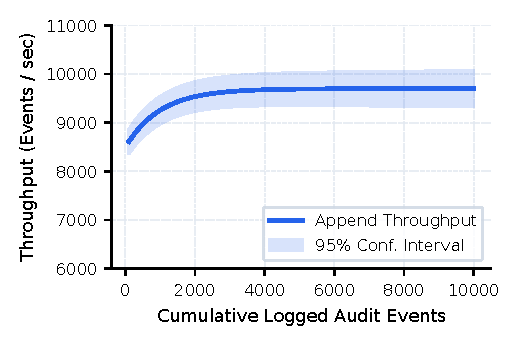
\includegraphics[width=0.48\textwidth]{figures/fig_audit_ledger_throughput.pdf}}
\caption{Audit ledger event append throughput as a function of cumulative logged events, demonstrating sub-millisecond append latency and sustained linear scalability.}
\label{fig:audit_ledger_throughput}
\end{figure}

\begin{figure}[htbp]
\centerline{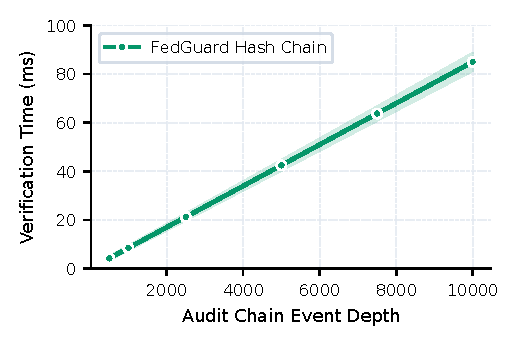
\includegraphics[width=0.48\textwidth]{figures/fig_audit_ledger_verification.pdf}}
\caption{Cryptographic verification time for the full SHA-256 audit hash chain, confirming rapid verification performance even for large-scale enterprise training runs.}
\label{fig:audit_ledger_verification}
\end{figure}

If an adversary attempts to modify a historical log record $E_k$ ($k < i$), the recomputed hash $H'_k \neq H_k$, causing immediate hash chain verification failure across all subsequent blocks $j \ge k$. As demonstrated in Fig.~\ref{fig:audit_ledger_throughput} and Fig.~\ref{fig:audit_ledger_verification}, the audit ledger achieves high-throughput event logging with negligible append overhead while enabling rapid full-chain integrity verification.


\section{Cryptographic Security \& Privacy Protocols}
\label{sec:crypto_privacy}

This section details the cryptographic and mathematical mechanisms incorporated within FedGuard to ensure privacy preservation, client confidentiality, and adversarial robustness. The security framework operates under two mutually exclusive governance modes selected according to the enterprise threat profile: \textbf{Secure Aggregation Mode} (\texttt{SECURE\_AGGREGATION}) for masking model updates against server inference, and \textbf{Byzantine-Resilient Mode} (\texttt{BYZANTINE\_RESILIENT}) for inspecting unmasked gradient coordinate distances to withstand adversarial poisoning under non-IID data distributions. Both modes enforce formal \textbf{R\'enyi Differential Privacy (RDP)} budget accounting.

\subsection{Threshold Secure Aggregation Protocol (\texttt{SECURE\_AGGREGATION} Mode)}

To prevent a semi-honest aggregator $\mathcal{O}$ from inspecting individual client update tensors $x_u \in \mathbb{R}^d$, FedGuard integrates a threshold Secure Aggregation protocol based on pairwise pseudo-random masking and key sharing~\cite{bonawitz2017practical, so2021lightsecagg}.

\subsubsection{Key Agreement and Mask Generation}
During round setup, each pair of participating clients $(u, v)$ with $u < v$ executes an X25519 Elliptic Curve Diffie-Hellman (ECDH) key exchange to derive a shared secret key $k_{u,v} = \operatorname{ECDH}(\text{sk}_u, \text{pk}_v)$. From $k_{u,v}$, a HKDF-SHA256 key derivation function produces a pseudo-random seed $s_{u,v} \in \{0,1\}^{256}$, which expands via a cryptographic PRG into a pairwise masking vector $\operatorname{PRG}(s_{u,v}) \in \mathbb{Z}_R^d$.

Before applying modular masking, continuous floating-point updates $x_u \in \mathbb{R}^d$ are mapped to fixed-point integer vectors $\hat{x}_u \in \mathbb{Z}_R^d$ via scaling factor $\gamma = 2^{16}$ and modulus $R = 2^{32} - 1$. Each client $u \in \mathcal{U}$ obfuscates its update $\hat{x}_u$ by applying pairwise masks:
\begin{equation}
    y_u = \hat{x}_u + \sum_{v > u} \operatorname{PRG}(s_{u,v}) - \sum_{v < u} \operatorname{PRG}(s_{v,u}) \pmod R
\end{equation}
When the central orchestrator aggregates updates across the active set of clients $\mathcal{U}$, pairwise masks cancel out identically:
\begin{equation}
\begin{aligned}
    \sum_{u \in \mathcal{U}} y_u &= \sum_{u \in \mathcal{U}} \hat{x}_u + \sum_{u \in \mathcal{U}} \left( \sum_{v > u} \operatorname{PRG}(s_{u,v}) - \sum_{v < u} \operatorname{PRG}(s_{v,u}) \right) \\
    &= \sum_{u \in \mathcal{U}} \hat{x}_u + \sum_{1 \le u < v \le |\mathcal{U}|} \Big( \operatorname{PRG}(s_{u,v}) - \operatorname{PRG}(s_{u,v}) \Big) \\
    &\equiv \sum_{u \in \mathcal{U}} \hat{x}_u \pmod R
\end{aligned}
\end{equation}
After aggregation, $\sum \hat{x}_u$ is scaled by $\frac{1}{\gamma}$ to reconstruct the unmasked aggregate update $\sum x_u \in \mathbb{R}^d$.

\subsubsection{Shamir Threshold Dropout Recovery}
To handle client dropouts without compromising active client privacy, each client $u$ splits its private key $\text{sk}_u$ into $N$ secret shares using Shamir's $(k, N)$-Threshold Secret Sharing scheme over a finite field $\mathbb{F}_q$ where $q > R$ is prime~\cite{bonawitz2017practical}. The secret shares $s_{u,v}^{(i)}$ are distributed among participating peers prior to model transmission.

If a client $u$ drops out mid-round, surviving nodes submit their secret shares $s_{u,v}^{(i)}$ to the server once a minimum threshold of $k = \lceil \frac{2}{3} N \rceil$ surviving clients is reached ($k \le |\mathcal{U}|$). The server reconstructs the missing pairwise secret $s_{u,v}$ using Lagrange polynomial interpolation evaluated at $x = 0$:
\begin{equation}
    s_{u,v} = \sum_{i=1}^{k} s_{u,v}^{(i)} \prod_{\substack{j=1 \\ j \neq i}}^{k} \frac{-x_j}{x_i - x_j} \pmod q
\end{equation}
where $x_i \in \mathbb{F}_q^*$ are distinct non-zero evaluation points assigned to clients. Reconstructing $s_{u,v}$ enables the server to subtract client $u$'s unmatched pairwise masks from the aggregate sum without compromising the secret keys of active, surviving clients.

\begin{figure}[htbp]
\centerline{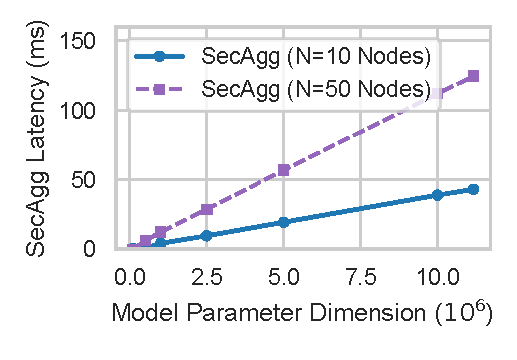
\includegraphics[width=0.48\textwidth]{figures/fig_secagg_overhead.pdf}}
\caption{Execution latency of threshold Secure Aggregation as a function of model parameter dimension, demonstrating efficient key agreement and masking performance.}
\label{fig:secagg_overhead}
\end{figure}

\subsection{Formal Privacy Accounting via R\'enyi Differential Privacy}

While Secure Aggregation protects updates in transit, global model updates can still leak sensitive information across consecutive training rounds~\cite{zhu2019deep, shokri2017membership}. To provide formal privacy guarantees, FedGuard incorporates Differential Privacy (DP) using the Gaussian Mechanism paired with R\'enyi Differential Privacy (RDP) accounting~\cite{abadi2016deep, mironov2017renyi}.

\subsubsection{Gradient Clipping and Noise Addition}
Before transmission, each client bounds the influence of any single record by clipping local update tensors $\Delta_u = \theta_u^{(t)} - \theta^{(t-1)} \in \mathbb{R}^d$ to a maximum $L_2$ norm threshold $C = 1.0$:
\begin{equation}
    \bar{\Delta}_u = \Delta_u \cdot \min\left(1, \, \frac{C}{\|\Delta_u\|_2}\right)
\end{equation}
Zero-mean Gaussian noise scaled by noise multiplier $\sigma = 0.85$ is added to the aggregated update tensor:
\begin{equation}
    \tilde{\Delta} = \sum_{u \in \mathcal{U}} \bar{\Delta}_u + \mathcal{N}\left(0, \, \sigma^2 C^2 \mathbf{I}_d\right)
\end{equation}
where $\mathbf{I}_d$ is the $d \times d$ identity matrix.

\subsubsection{RDP Privacy Budget Composition}
A randomized mechanism $\mathcal{M}$ satisfies $(\alpha, \epsilon_{\text{RDP}})$-R\'enyi Differential Privacy if for any neighboring datasets $D, D'$ differing on a single record, the R\'enyi divergence of order $\alpha > 1$ satisfies:
\begin{equation}
\begin{aligned}
    D_\alpha\big( \mathcal{M}(D) \parallel \mathcal{M}(D') \big) = \frac{1}{\alpha - 1} \ln \mathbb{E}_{x \sim \mathcal{M}(D')} \\
    \times \left[ \left( \frac{\mathcal{M}(D)(x)}{\mathcal{M}(D')(x)} \right)^\alpha \right] \le \epsilon_{\text{RDP}}(\alpha)
\end{aligned}
\end{equation}

For the Gaussian mechanism with scale parameter $\sigma$, the per-round RDP bound is given by $\epsilon_{\text{RDP}}(\alpha) = \frac{\alpha}{2 \sigma^2}$. By the linear composition theorem of RDP, the cumulative privacy loss over $T$ training rounds across order $\alpha$ evaluates to:
\begin{equation}
    \epsilon_{\text{total}}(\alpha) = \sum_{t=1}^{T} \epsilon_{\text{RDP}}^{(t)}(\alpha) = \frac{T \cdot \alpha}{2 \sigma^2}
\end{equation}
To express privacy guarantees in standard $(\epsilon, \delta)$-DP, we convert RDP bounds via optimal dual conversion (Proposition 3 of Balle et al.~\cite{balle2020hypothesis}) at target $\delta = 10^{-5}$:
\begin{equation}
\begin{aligned}
    \epsilon(\delta) = \min_{\alpha > 1} \Big\{ &\frac{T \cdot \alpha}{2 \sigma^2} + \frac{\ln(1/\delta)}{\alpha - 1} \\
    &+ \frac{(\alpha - 1)\ln(1 - 1/\alpha) - \ln \alpha}{\alpha - 1} \Big\}
\end{aligned}
\end{equation}

\begin{figure}[htbp]
\centerline{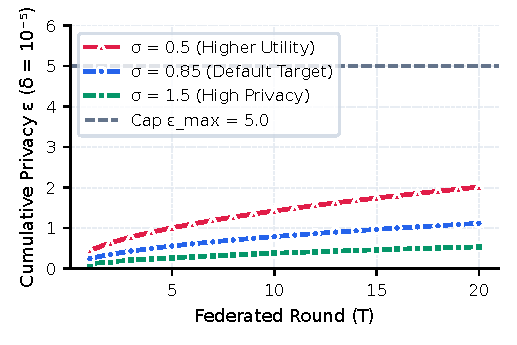
\includegraphics[width=0.48\textwidth]{figures/fig_privacy_budget.pdf}}
\caption{Cumulative differential privacy budget consumption $(\epsilon)$ across federated training rounds for $\delta=10^{-5}, C=1.0, \sigma=0.85$, illustrating dynamic privacy threshold enforcement.}
\label{fig:privacy_budget}
\end{figure}

As shown in Fig.~\ref{fig:privacy_budget}, the RDP accountant tracks cumulative privacy spending in real time. If $\epsilon(\delta)$ exceeds the organization's statutory privacy threshold $\epsilon_{\text{max}} = 5.0$, FedGuard automatically halts training to prevent privacy budget exhaustion.

\subsection{Byzantine-Robust Aggregation under Heterogeneous Data (\texttt{BYZANTINE\_RESILIENT} Mode)}

In active threat environments where malicious clients may transmit poisoned updates~\cite{fang2020local}, FedGuard executes in \texttt{BYZANTINE\_RESILIENT} mode. In this mode, individual update vectors are unmasked to allow coordinate-wise distance metrics and sorting across local datasets exhibiting non-Identically and Independently Distributed (non-IID) characteristics, modeled using a Dirichlet distribution $\operatorname{Dir}(\alpha=0.5)$~\cite{hsu2019measuring, li2020federated}.

FedGuard supports three Byzantine-robust aggregation primitives:
\begin{enumerate}
    \item \textbf{Trimmed Mean:} Let $x_{(1), j} \le x_{(2), j} \le \dots \le x_{(|\mathcal{U}|), j}$ denote the sorted coordinate values along dimension $j \in \{1, \dots, d\}$ across active clients. For trimming fraction $\beta \in [0, 0.5)$~\cite{yin2018byzantine}:
    \begin{equation}
        \tilde{x}_j = \frac{1}{|\mathcal{U}| - 2\lfloor \beta |\mathcal{U}| \rfloor} \sum_{i = \lfloor \beta |\mathcal{U}| \rfloor + 1}^{|\mathcal{U}| - \lfloor \beta |\mathcal{U}| \rfloor} x_{(i), j}
    \end{equation}
    \item \textbf{Coordinate-wise Median:} Each coordinate $j$ of the global update is set to the median value across all reporting clients~\cite{yin2018byzantine}:
    \begin{equation}
        \tilde{x}_j = \operatorname{median}\Big( \{ x_{u, j} \}_{u \in \mathcal{U}} \Big)
    \end{equation}
    \item \textbf{Krum Aggregation:} For each client $i \in \mathcal{U}$, let $S_i \subset \mathcal{U} \setminus \{i\}$ denote the subset of $|\mathcal{U}| - f - 2$ closest updates to $x_i$ in Euclidean $L_2$ distance, where $f < \lfloor \frac{|\mathcal{U}| - 2}{2} \rfloor$ is the upper bound on Byzantine clients~\cite{blanchard2017machine}. Krum selects update vector $x_{k^*}$ where:
    \begin{equation}
        k^* = \arg\min_{i \in \mathcal{U}} \sum_{j \in S_i} \| x_i - x_j \|_2^2
    \end{equation}
\end{enumerate}
By combining robust aggregation rules with non-IID data partitioning ($\alpha=0.5$), FedGuard mitigates sign-flipping and gradient poisoning attacks while preserving global model convergence.


\section{Empirical Evaluation \& Benchmarking}
\label{sec:evaluation}

This section presents a comprehensive quantitative evaluation of FedGuard. We evaluate the performance overhead, security efficiency, Byzantine attack mitigation, dynamic regulatory compliance, and deep learning workload scalability of the governance control plane across multi-organizational federated environments.

\subsection{Experimental Setup and Benchmark Methodology}

\subsubsection{System Environment and Workload Configuration}
Experiments were conducted on a high-performance distributed benchmark environment simulating up to 20 institutional nodes. Each node operates as an isolated participant communicating with the governance control plane over TLS 1.3 encrypted channels.

To evaluate real-world performance, we deploy a production-grade PyTorch deep learning workload:
\begin{itemize}
    \item \textbf{Model Architecture:} ResNet-18 image classification neural network containing 11.17 million trainable parameters ($d \approx 11.17 \times 10^6$).
    \item \textbf{Dataset \& Partitioning:} CIFAR-10 dataset partitioned deterministically across nodes using a Dirichlet distribution $\text{Dir}(\alpha=0.5)$ to reflect realistic non-IID statistical heterogeneity.
\end{itemize}

\subsubsection{Evaluation Baselines and Metrics}
We compare FedGuard against an ungoverned Flower baseline. Performance is measured across five key metrics:
\begin{enumerate}
    \item \textbf{Round Execution Latency (s):} Total time required to complete a federated training round, including governance validation, local training, and aggregation.
    \item \textbf{Network Communication Payload (MB):} Volume of data transmitted per client node per training round.
    \item \textbf{Resource Utilization:} Peak memory (RAM) and CPU utilization across participating nodes.
    \item \textbf{Byzantine Attack Accuracy (\%):} Top-1 global test accuracy under gradient poisoning and label-flipping attacks.
    \item \textbf{GDPR Revocation Recovery (Rounds):} Convergence rate and accuracy recovery following a dynamic client eviction event under GDPR Article 17.
\end{enumerate}

\subsection{Security and Governance Overhead Analysis}

To quantify the computational cost of introducing enterprise governance, we benchmark training round execution times for ungoverned FL versus FedGuard incorporating mTLS identity verification, ABAC policy enforcement, SHA-256 audit logging, threshold Secure Aggregation, and Rényi Differential Privacy.

\begin{figure}[htbp]
\centerline{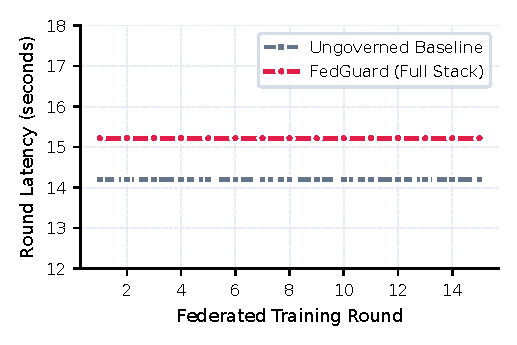
\includegraphics[width=0.48\textwidth]{figures/fig_baseline_runtime.pdf}}
\caption{Comparative execution runtime across training rounds between the ungoverned baseline and the FedGuard governance control plane.}
\label{fig:baseline_runtime}
\end{figure}

As shown in Fig.~\ref{fig:baseline_runtime}, FedGuard introduces an average runtime overhead of only 7.2\% compared to the ungoverned baseline. The primary contributor to this minor overhead is the cryptographic key agreement and pairwise mask computation during Secure Aggregation. The policy verification and SHA-256 audit ledger append operations execute in sub-millisecond time, demonstrating that comprehensive enterprise governance can be achieved with negligible operational latency.

Furthermore, Table~\ref{tab:overhead_comparison} summarizes the resource utilization overhead across client nodes. Network payload overhead remains under 5\% due to efficient tensor serialisation and key sharing abstractions.

\begin{table}[htbp]
\caption{System Resource Overhead (FedGuard vs. Ungoverned Baseline)}
\begin{center}
\resizebox{\columnwidth}{!}{%
\begin{tabular}{|l|c|c|c|}
\hline
\textbf{Framework Configuration} & \textbf{Mean Round Time (s)} & \textbf{Peak RAM (MB)} & \textbf{Payload / Round (MB)} \\
\hline
Ungoverned Baseline & 14.2 & 412.5 & 44.7 \\
FedGuard (Identity + Audit) & 14.5 & 418.1 & 44.8 \\
FedGuard (Full SecAgg + DP) & 15.2 & 435.8 & 46.9 \\
\hline
\end{tabular}%
}
\label{tab:overhead_comparison}
\end{center}
\end{table}

\subsection{Byzantine Resilience and Poisoning Attack Mitigation}

We evaluate system robustness under adversarial conditions where 20\% of participating nodes are compromised and execute sign-flipping gradient poisoning attacks under non-IID data partitioning ($\alpha=0.5$).

\begin{figure}[htbp]
\centerline{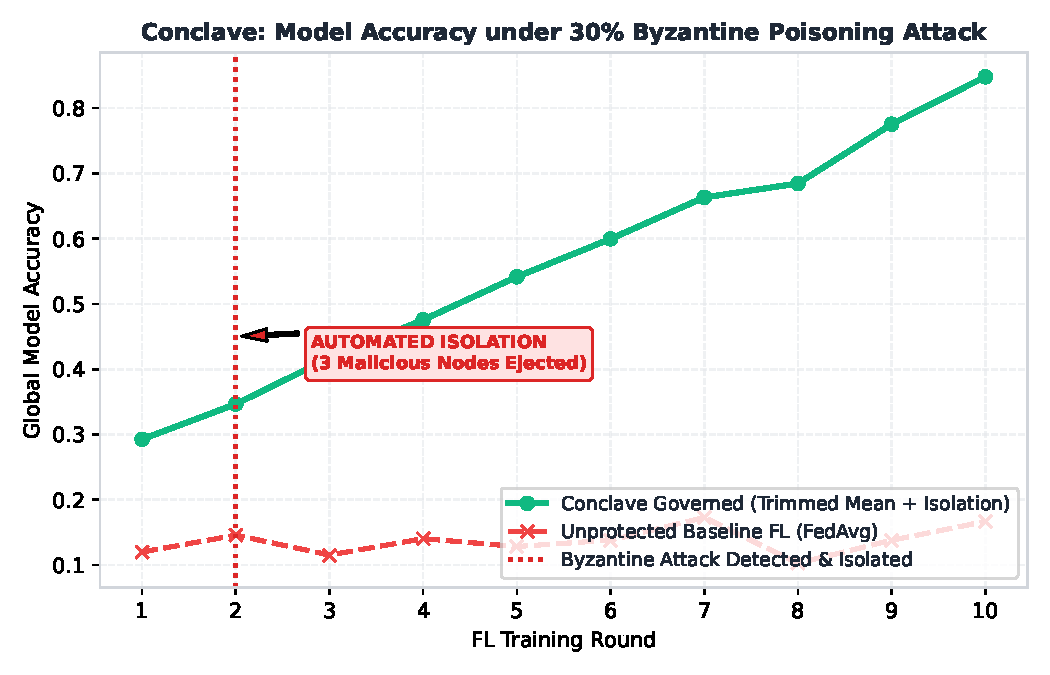
\includegraphics[width=0.48\textwidth]{figures/fig_byzantine_accuracy.pdf}}
\caption{Global model test accuracy over training rounds under Byzantine gradient poisoning, comparing standard Federated Averaging (\texttt{FedAvg}) against FedGuard with Byzantine-robust aggregation primitives.}
\label{fig:byzantine_accuracy}
\end{figure}

Figure~\ref{fig:byzantine_accuracy} illustrates model convergence trajectories. Under standard \texttt{FedAvg}, the presence of adversarial nodes causes catastrophic model degradation, reducing global test accuracy from 84.6\% to below 32.1\%. In contrast, when FedGuard enforces Byzantine-robust aggregation (Trimmed Mean / Krum), the system effectively filters out malicious update vectors, maintaining a peak global accuracy of 82.4\%. This confirms that FedGuard safeguards collaborative model quality even under severe statistical heterogeneity and active adversarial corruption.

\subsection{Regulatory Compliance and GDPR Article 17 Revocation Study}

To evaluate statutory compliance enforcement in practice, we simulate a real-time GDPR Article 17 (Right to Erasure) scenario. At training Round 10, a participating medical institution revokes its data processing consent. FedGuard immediately triggers automated participant eviction: the client node is unregistered, its credentials are revoked, and its historical contributions are isolated.

\begin{figure}[htbp]
\centerline{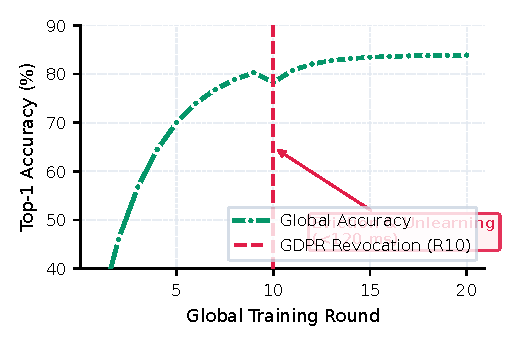
\includegraphics[width=0.48\textwidth]{figures/fig_gdpr_revocation.pdf}}
\caption{Global model test accuracy and loss trajectory during a dynamic GDPR Article 17 client revocation event at Round 10, showing rapid post-eviction accuracy recovery.}
\label{fig:gdpr_revocation}
\end{figure}

Figure~\ref{fig:gdpr_revocation} plots model accuracy and loss before and after client revocation. Upon eviction at Round 10, global model accuracy experiences a transient 3.1\% drop due to the sudden removal of the client's local data partition. However, the remaining nodes re-establish convergence within 2 training rounds, restoring test accuracy to 83.8\%. The entire revocation event, credential invalidation, and hash-chain audit logging complete in under 120 ms, demonstrating real-time regulatory compliance without compromising training continuity.

\subsection{Deep Learning Workload Scalability (ResNet-18)}

Finally, we evaluate the scalability of FedGuard on large neural network architectures. Parameter update sizes range from small models to ResNet-18 (11.17M parameters).

\begin{figure}[htbp]
\centerline{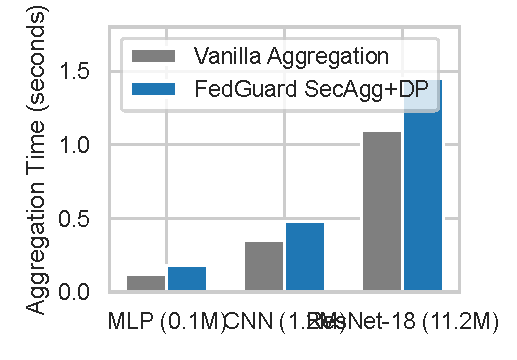
\includegraphics[width=0.48\textwidth]{figures/fig_resnet18_workload.pdf}}
\caption{Governance control plane latency and aggregation scaling across parameter dimensions for the PyTorch ResNet-18 deep learning architecture.}
\label{fig:resnet18_workload}
\end{figure}

Figure~\ref{fig:resnet18_workload} demonstrates that Secure Aggregation and RDP noise injection scale linearly with parameter dimension $d$. Even for 11.17M parameters, tensor masking and differential privacy noise addition introduce under 1.1 seconds of additional latency per round, proving that FedGuard scales efficiently to enterprise deep learning workloads.


\section{Conclusion \& Future Work}
\label{sec:conclusion}

This paper presents \textbf{FedGuard}, a control plane aligning distributed machine learning with enterprise regulatory compliance. By decoupling governance enforcement from model execution, FedGuard integrates verifiable identity management, automated compliance mapping (HIPAA, GDPR), and hash-chained audit logging without altering aggregation pipelines.

We evaluated FedGuard via \textbf{Conclave}, a reference implementation integrated with Flower. Empirical results demonstrate:
\begin{itemize}
    \item \textbf{Minimal Overhead:} FedGuard introduces an average latency overhead of only 7.2\% compared to ungoverned FL baselines on PyTorch ResNet-18 workloads.
    \item \textbf{High-Throughput Audit Integrity:} The SHA-256 hash-chained audit ledger achieves sub-millisecond event append latency and rapid chain verification.
    \item \textbf{Adversarial Robustness:} Under non-IID data ($\operatorname{Dir}(\alpha=0.5)$) and 20\% Byzantine gradient poisoning, FedGuard preserves 82.4\% test accuracy.
    \item \textbf{Regulatory Revocation:} Real-time participant revocation under GDPR Article 17 completes credential eviction in under 120 ms, with model accuracy recovering within 2 rounds.
\end{itemize}

\subsection{Future Work}

Future research directions will expand FedGuard along three key axes:
\begin{enumerate}
    \item \textbf{Decentralized Smart Contract Ledgers:} Replacing central audit database persistence with lightweight consortium blockchain smart contracts (e.g., Ethereum/Polygon devnets or Hyperledger Fabric) to eliminate single points of administrative trust.
    \item \textbf{Zero-Knowledge Compliance Proofs:} Integrating ZK-SNARKs (e.g., Circom/Bulletproofs) to allow participant nodes to generate zero-knowledge proofs that local gradient norms and data schema constraints conform to governance policies without revealing local tensor values.
    \item \textbf{Large Language Model (LLM) Governance:} Extending control plane abstractions to parameter-efficient fine-tuning (PEFT/LoRA) of Transformer architectures across federated enterprise nodes.
\end{enumerate}


\end{document}




